%%%%%%%%%%%%%%%%%%%%%%%%%%%% Define Article %%%%%%%%%%%%%%%%%%%%%%%%%%%%%%%%%%
\documentclass[nobib, openany, justified, a4paper, 14pt]{tufte-book}
%%%%%%%%%%%%%%%%%%%%%%%%%%%%%%%%%%%%%%%%%%%%%%%%%%%%%%%%%%%%%%%%%%%%%%%%%%%%%%%

%%%%%%%%%%%%%%%%%%%%%%%%%%%%% Citations %%%%%%%%%%%%%%%%%%%%%%%%%%%%%%%%%%%%%%%
%\usepackage[utf8]{inputenc}
\usepackage[style=authoryear-icomp]{biblatex}
%\usepackage[style=apa]{biblatex}
\addbibresource{/Users/ubd/Bibliotheca/bib.bib}
%%%%%%%%%%%%%%%%%%%%%%%%%%%%%%%%%%%%%%%%%%%%%%%%%%%%%%%%%%%%%%%%%%%%%%%%%%%%%%%

%%%%%%%%%%%%%%%%%%%%%%%%%%%%% Using Packages %%%%%%%%%%%%%%%%%%%%%%%%%%%%%%%%%%
\usepackage{newunicodechar}
\newunicodechar{🦜}{[parrot]}
\PassOptionsToPackage{prologue,dvipsnames}{xcolor}
\sloppy  % globally
\usepackage{geometry}
\usepackage{graphicx}
\usepackage{amssymb}
\usepackage{amsmath}
\usepackage{amsthm}
\usepackage{empheq}
\usepackage{mdframed}
\usepackage{booktabs}
\usepackage{lipsum}
\usepackage{graphicx}
\usepackage{color}
\usepackage{psfrag}
\usepackage{pgfplots}
\usepackage{bm}
\usepackage{epigraph}
\usepackage{titlesec}
\usepackage{tcolorbox}
\usepackage{csquotes}
\usepackage{pifont}
\usepackage{enumitem,amssymb}
% \usepackage{spoton} % adds \todo functionality I hope
%%%%%%%%%%%%%%%%%%%%%%%%%%%%%%%%%%%%%%%%%%%%%%%%%%%%%%%%%%%%%%%%%%%%%%%%%%%%%%%

% Other Settings

%%%%%%%%%%%%%%%%%%%%%%%%%% Page Setting %%%%%%%%%%%%%%%%%%%%%%%%%%%%%%%%%%%%%%%

%%%%%%%%%%%%%%%%%%%%%%%%%% Define some useful colors %%%%%%%%%%%%%%%%%%%%%%%%%%
\definecolor{maroon}{RGB}{128,0,0} %hlred
\definecolor{MAROON}{RGB}{128,0,0} %hlred
\definecolor{deepBlue}{RGB}{61,124,222} %url-links
\definecolor{deepGreen}{RGB}{26,111,0} %citations
\definecolor{ocre}{RGB}{243,102,25}
\definecolor{mygray}{RGB}{243,243,244}
\definecolor{shallowGreen}{RGB}{235,255,255}
\definecolor{shallowBlue}{RGB}{235,249,255}
\definecolor{mediumpersianBlue}{rgb}{0.0, 0.4, 0.65}
\definecolor{persianBlue}{rgb}{0.11, 0.22, 0.73}
\definecolor{persianGreen}{rgb}{0.0, 0.65, 0.58}
\definecolor{persianRed}{rgb}{0.8, 0.2, 0.2}
\definecolor{debianRed}{rgb}{0.84, 0.04, 0.33}
%%%%%%%%%%%%%%%%%%%%%%%%%%%%%%%%%%%%%%%%%%%%%%%%%%%%%%%%%%%%%%%%%%%%%%%%%%%%%%%

%%%%%%%%%%%%%%%%%%%%%%%%%% Indentation Settings %%%%%%%%%%%%%%%%%%%%%%%%%%%%%%%
\makeatletter
% Paragraph indentation and separation for normal text
\renewcommand{\@tufte@reset@par}{%
	\setlength{\RaggedRightParindent}{0pc}%1.0
	\setlength{\JustifyingParindent}{0pc}%1.0
	\setlength{\parindent}{1pc}%1pc
	\setlength{\parskip}{5pt}%0pt
}
\@tufte@reset@par

% Paragraph indentation and separation for marginal text
\renewcommand{\@tufte@margin@par}{%
	\setlength{\RaggedRightParindent}{0pc}%0.5pc
	\setlength{\JustifyingParindent}{0pc}%0.5pc
	\setlength{\parindent}{0.5pc}%
	\setlength{\parskip}{5pt}%0pt
}
\makeatother



%%%%%%%%%%%%%%%%%%%%%%%%%% Define an orangebox command %%%%%%%%%%%%%%%%%%%%%%%%
%o\usepackage[most]{tcolorbox}

\newtcolorbox{orangebox}{
	colframe=ocre,
	colback=mygray,
	boxrule=0.8pt,
	arc=0pt,
	left=2pt,
	right=2pt,
	width=\linewidth,
	boxsep=4pt
}


\newtcolorbox{redbox}{
	colframe=red,
	boxrule=0.8pt,
	arc=0pt,
	left=2pt,
	right=2pt,
	width=\linewidth,
	boxsep=4pt
}
%%%%%%%%%%%%%%%%%%%%%%%%%%%%%%%%%%%%%%%%%%%%%%%%%%%%%%%%%%%%%%%%%%%%%%%%%%%%%%%

%%%%%%%%%%%%%%%%%%%%%%%%%%%% English Environments %%%%%%%%%%%%%%%%%%%%%%%%%%%%%
\newtheoremstyle{mytheoremstyle}{3pt}{3pt}{\normalfont}{0cm}{\rmfamily\bfseries}{}{1em}{{\color{black}\thmname{#1}~\thmnumber{#2}}\thmnote{\,--\,#3}}
\newtheoremstyle{myproblemstyle}{3pt}{3pt}{\normalfont}{0cm}{\rmfamily\bfseries}{}{1em}{{\color{black}\thmname{#1}~\thmnumber{#2}}\thmnote{\,--\,#3}}
\theoremstyle{mytheoremstyle}
\newmdtheoremenv[linewidth=1pt,backgroundcolor=shallowGreen,linecolor=deepGreen,leftmargin=0pt,innerleftmargin=20pt,innerrightmargin=20pt,]{theorem}{Theorem}[section]
\theoremstyle{mytheoremstyle}
\newmdtheoremenv[linewidth=1pt,backgroundcolor=shallowBlue,linecolor=deepBlue,leftmargin=0pt,innerleftmargin=20pt,innerrightmargin=20pt,]{definition}{Definition}[section]
\theoremstyle{myproblemstyle}
\newmdtheoremenv[linecolor=black,leftmargin=0pt,innerleftmargin=10pt,innerrightmargin=10pt,]{problem}{Problem}[section]
%%%%%%%%%%%%%%%%%%%%%%%%%%%%%%%%%%%%%%%%%%%%%%%%%%%%%%%%%%%%%%%%%%%%%%%%%%%%%%%

%%%%%%%%%%%%%%%%%%%%%%%%%%%%%%% Plotting Settings %%%%%%%%%%%%%%%%%%%%%%%%%%%%%
\usepgfplotslibrary{colorbrewer}
\pgfplotsset{width=8cm,compat=1.9}
%%%%%%%%%%%%%%%%%%%%%%%%%%%%%%%%%%%%%%%%%%%%%%%%%%%%%%%%%%%%%%%%%%%%%%%%%%%%%%%

%%%%%%%%%%%%%%%%%%%%%%%%%%%%%%% MISC %%%%%%%%%%%%%%%%%%%%%%%%%%%%%%%%%%%%%%%%%%
\usepackage[acronym]{glossaries}
\usepackage{hyperref} % Setup: https://www.overleaf.com/learn/latex/Hyperlinks
\hypersetup{
	colorlinks=true,
	%citecolor=deepGreen,
	citecolor=maroon,
	linkcolor=persianBlue,
	filecolor=persianGreen,
	urlcolor=persianBlue,
	pdfpagemode=FullScreen,
}

%%%%%%%%%%%%%%%%%%%%%%%%%%%%%%%%%%%%%%%%%%%%%%%%%%%%%%%%%%%%%%%%%%%%%%%%%%%%%%%
\setcounter{tocdepth}{2}
\setcounter{secnumdepth}{2}

\newcommand{\hlred}[1]{\textcolor{Maroon}{#1}} % Print text in maroon
\newcommand{\hlgreen}[1]{\textcolor{persianGreen}{#1}} % Print text in green
\newcommand{\hlocre}[1]{\textcolor{ocre}{#1}} % Print text in green

\newenvironment{greenenv}{\color{Green}}{\ignorespacesafterend}  % Create green environment
\newenvironment{commentenv}{\color{ocre}}{\ignorespacesafterend}  % Create comment environment


\titleformat{\part}[display]
{\filleft\fontsize{40}{40}\selectfont\scshape}
{\fontsize{90}{90}\selectfont\thepart}
{20pt}
{\thispagestyle{epigraph}}

\setlength\epigraphwidth{.6\textwidth}

%\makeatletter
%\epigraphhead
%{\let\@evenfoot}
%{\let\@oddfoot\@empty\let\@evenfoot}
%{}{}
%\makeatother


%%%%%%%%%%%%%%%%%%%%%%%%%%%%%%%%%%%%%%%%%%%%%%%%%%%%%%%%%%%%%%%%%%%%%%%%%%%%%%%
%TODO LIST
\newlist{todolist}{itemize}{2}
\setlist[todolist]{label=$\square$}
\newcommand{\cmark}{\ding{51}}%
\newcommand{\xmark}{\ding{55}}%
\newcommand{\done}{\rlap{$\square$}{\raisebox{2pt}{\large\hspace{1pt}\cmark}}%
	\hspace{-2.5pt}}
\newcommand{\wontfix}{\rlap{$\square$}{\large\hspace{1pt}\xmark}}

%%%%%%%%%%%%%%%%%%%%%%%%%%%%%%%%%%%%%%%%%%%%%%%%%%%%%%%%%%%%%%%%%%%%%%%%%%%%%%%
\newcommand{\greensquare}{\marginnote{\fcolorbox{green}{green}{\rule{0pt}{3mm}\rule{3mm}{0pt}}\quad}}
\newcommand{\yellowsquare}{\marginnote{\fcolorbox{yellow}{yellow}{\rule{0pt}{3mm}\rule{3mm}{0pt}}\quad}}
\newcommand{\redsquare}{\marginnote{\fcolorbox{red}{red}{\rule{0pt}{3mm}\rule{3mm}{0pt}}\quad}}



\usepackage{epigraph}
\usepackage{titlesec}

\setcounter{tocdepth}{2}
\setcounter{secnumdepth}{2}

\newcommand{\hlred}[1]{\textcolor{Maroon}{#1}} % Print text in maroon

\titleformat{\part}[display]
  {\filleft\fontsize{40}{40}\selectfont\scshape}
  {\fontsize{90}{90}\selectfont\thepart}
  {20pt}
  {\thispagestyle{epigraph}}

\setlength\epigraphwidth{.6\textwidth}

\makeatletter
\xpatchcmd\epigraphhead
 {\let\@evenfoot}
 {\let\@oddfoot\@empty\let\@evenfoot}
 {}{}
\makeatother

%%%%%%%%%%%%%%%%%%%%%%%%%%%%%%% Title & Author %%%%%%%%%%%%%%%%%%%%%%%%%%%%%%%%
\title{Derepresentative \\ Claims: \\ \large{Abundance and Lack of Representation in Gezi Assemblage}}
\author{Utku B. Demir}
%%%%%%%%%%%%%%%%%%%%%%%%%%%%%%%%%%%%%%%%%%%%%%%%%%%%%%%%%%%%%%%%%%%%%%%%%%%%%%%

\begin{document}
    \maketitle
    \tableofcontents
    \newpage

\chapter{Introduction}

In recent years, the landscape of political protest has undergone a significant transformation, marked by a surge in social movements that challenge traditional notions of representation and leadership. This shift has been especially pronounced in movements like the Gezi Resistance in Turkey, which offer a unique lens through which to examine contemporary issues of political representation, inclusivity, and organizational structure. The Gezi Park protests, which began as a local environmental campaign to protect a small park in Istanbul, rapidly evolved into a broader movement against authoritarian governance and social injustices, drawing diverse groups into a complex web of resistance.

This paper aims to deliver a critique of the claimed decentralization in contemporary political movements by using the Gezi Resistance as a case study. Through the theoretical frameworks of Michael Saward's "Representative Claims" and Samuel Hayat's "Unrepresentative Claims," this analysis explores how the Gezi movement embodied a rich political discourse that both challenged and adhered to conventional forms of representation. Saward’s theory provides a foundation for understanding the performative nature of representation within social movements, highlighting the dynamic and contested processes that underpin political claims. Hayat’s concept of "unrepresentative claims" further complicates this picture, suggesting that the deliberate refusal to adopt traditional representative roles can serve both as a tool of authenticity and a source of internal conflict.

The discussion is structured around three core arguments. Firstly, the paper posits that the failure or avoidance of factionalization within the Gezi movement led to a collapse in its ability to develop a coherent political agenda. Secondly, it argues that unrepresentative claims, while fostering inclusivity, hinder the formation of a necessary referent that is essential for effective political mobilization and party building. Thirdly, the paper critiques Hardt and Negri’s theory of Assembly, which, while advocating for a leaderless organizational model, fails to account for the benefits of factionalization in enriching political discourse and fostering a more dynamic and robust democratic engagement.

By examining the Gezi Resistance through these theoretical lenses, this paper seeks to contribute to the broader discourse on representation in social movements, highlighting the tensions and contradictions that arise when traditional and non-traditional forms of political engagement intersect. The analysis underscores the importance of understanding the mechanisms of representation and the role of internal divisions in shaping the trajectory and outcomes of social movements in an increasingly interconnected and complex global political landscape.

\chapter{Theoretical Framework}

\section{Literature Review and Current Debates}
This paper examines the evolving nature of political representation in social movements, focusing on the Gezi Resistance as a case study. Key theoretical perspectives include Michael Saward's concept of "Representative Claims," Samuel Hayat's idea of "Unrepresentative Claims," and Michael Hardt and Antonio Negri's theory of Assembly.

Saward's framework posits that representation is a performative act, involving the continuous making and contesting of claims rather than being a static relationship. This approach helps us understand how various actors within social movements like Gezi attempt to position themselves as representatives, ven without formal electoral mechanisms \parencite[-]{saward2010}.

Hayat introduces "Unrepresentative Claims," where individuals or groups within social movements deliberately refuse to act as representatives for others, emphasizing personal authenticity over collective representation. This perspective challenges traditional notions of political representation, particularly in contexts with widespread distrust of established political institutions \parencite[1038-1043]{hayat2022}.

Hardt and Negri's concept of Assembly advocates for a leaderless, non-hierarchical model that prioritizes collective decision-making and inclusivity. While this model promotes direct participation, it also poses challenges in maintaining coherence and strategic direction, as seen in the Gezi Resistance \parencite[69]{hardt2017}.
\section{Methodology and Research Question}

The formulation of the research question is as follows.

\hlred{Research Question:} To what extent does the ability (and tendency) of initially leaderless, horizontally structured social movements like Gezi Resistance to factionalize affect their organizational performance?

This research question will be explored through the specific case study of the Gezi Resistance in Istanbul. The analysis will be guided by the following hypotheses:

\begin{enumerate} \item The collapse of the Gezi Resistance was directly caused by the failure or avoidance of the factionalization process among its supporters. \item An overreliance on unrepresentative claims leads to a failure in social movements to create diverse imaginaries (or distinct referents) that could facilitate the formation of different factions. \item Hardt and Negri's emphasis on effective organization and solidarity structures in Assembly is insufficient to generate new subjectivities without a robust factionalization process. \end{enumerate}

\chapter{Performative Claims and the Contemporary Construct}
%\epigraph{Well as, one judge said to the other, 'Be just and if you can't be just be arbitrary.' Regret cannot observe customary obscenities.\par\hspace*{\fill} -- \cite{burroughs1979}}

The current surge in popular protests across the globe has sparked a significant debate: are we witnessing a crisis of representative government, or is this a necessary evolution towards a more interconnected global society faced with increasingly complex issues? As the frequency and diversity of these protests grow, the traditional frameworks of representation and leadership are being challenged and redefined \parencite[see 1039]{hayat2022}. One of the primary difficulties in analyzing these social movements is the elusive nature of representation itself. Unlike the clear-cut representation seen in electoral politics, the representation within these movements is often ambiguous or entirely absent. This ambiguity reflects a growing dissatisfaction with Weberian forms of leadership, where the electorate is growing increasingly disillusioned with representative figures and the procedural norms of liberal democracies \parencite[see for example 5-14]{hardt2017}.

In this context, Michael Saward's concept of "Representative Claims" has emerged as a crucial framework for understanding the shifting dynamics of representation within social movements \parencite[-]{saward2010}. Rather than simply extending electoral representation into the public sphere or providing a rigid formula to validate representational legitimacy, Saward's approach is far more foundational. It seeks to uncover the underlying mechanisms of representation itself, highlighting how political presence is constituted and contested. At the heart of Saward's theory is the concept of the "representative claim." This involves a complex interplay between five elements: A maker of representations puts forward a subject which stands for an object that is related to a referent and is offered to an audience (ibid.).

Saward's model underscores the performative and inherently contested nature of representation, suggesting that it is never fully settled but always in a state of negotiation and reinterpretation \parencite[see 36-37]{saward2010}. By focusing on the mechanism rather than the meaning of representation, Saward's framework allows for a more nuanced analysis of the diverse contexts in which representative claims are made. It also highlights the fluidity and multiplicity of representation in contemporary social movements, where traditional forms of authority and legitimacy are continually being questioned and reimagined.

Building on Saward's concept, Samuel Hayat has recently introduced the idea of "unrepresentative claims," where individuals or leaders within social movements intentionally avoid acting as representatives for others and instead claim to speak solely for themselves. This idea is examined in the context of the French Yellow Vest movement, where participants and leaders often made such claims to reject traditional political representation, aiming to preserve authenticity and autonomy. The notion of unrepresentative claims challenges the conventional view of political representation, which typically involves speaking or acting on behalf of a group. Hayat argues that these claims expose the tension between the desire for genuine personal expression and the demands of collective representation, particularly in situations where there is widespread distrust of established political institutions. He differentiates between the negative and positive aspects of unrepresentative claims: Negative claims reject any formal mandate or representative role, thereby refusing to act on behalf of others, while positive claims occur when individuals present themselves as embodying particular identities or experiences, indirectly creating a form of representation through their own embodiment and self-presentation \parencite[see 1038-1043]{hayat2022}.

\begin{marginfigure}
  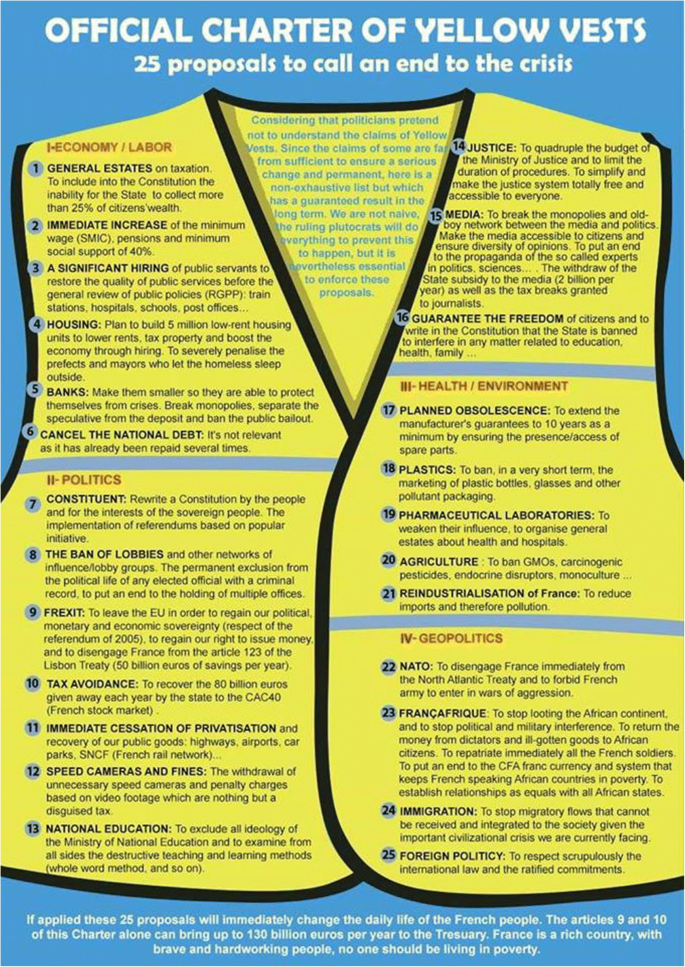
\includegraphics[scale=0.23]{gilets_jaunes.png}
  \caption{The official demands of Gilets Jaunes}\\
  \label{fig:gilets_jaunes}
\end{marginfigure}


Hayat's analysis is closely linked to the Yellow Vest Movement (Gilets Jaunes, see Figure \ref{fig
} for their initial demands), which serves as a prominent example of a social movement characterized by unrepresentative claims. The movement’s process demonstrated both immediate benefits and certain issues arising from the lack of any structured representation. The Yellow Vest Movement fundamentally rejected traditional forms of political representation, such as political parties and unions, and avoided formal leadership and organizational structures, presenting itself instead as a direct embodiment of the people. This approach was seen as a conscious "avoidance of institutional politics," allowing participants to assert that they represented the people as a whole, rather than any specific political group or faction \parencite[see especially 4-6]{hayat2024}. This stance also prevented \textbf{any form of factionalisation} within the movement, as there were no significant conflicts of interest beyond a quiet form of \textit{individual disagreements}, since everyone continued to claim to represent only themselves.

\begin{marginfigure}
  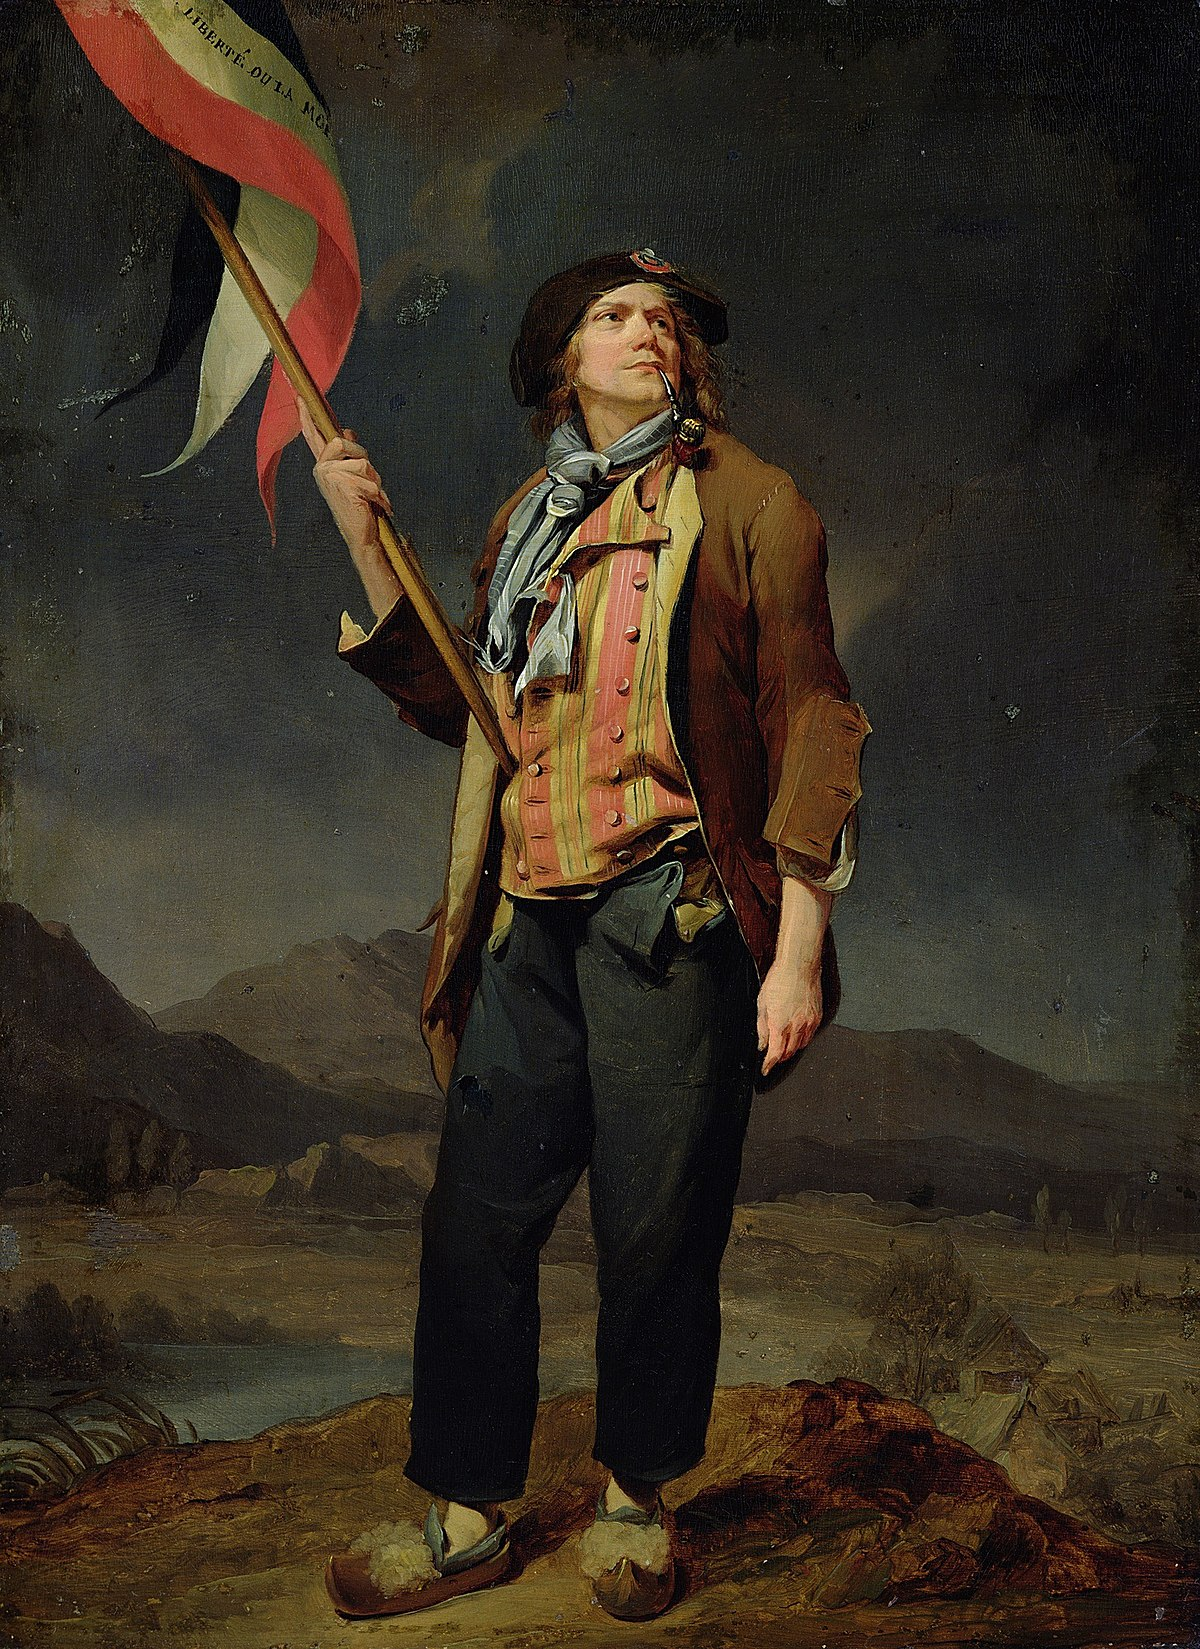
\includegraphics[scale=0.12]{Sans-culotte.jpg}
  \caption{A description of Sans-Culottes (without breeches); they were a radical and militant faction during the French Revolution, primarily composed of working-class Parisians, such as artisans, shopkeepers, but mostly simply laborers.}\\
  \label{fig:sans_culottes}
\end{marginfigure}

The Yellow Vest Movement also employed imagery and rhetoric from the French Revolution, such as references to the Sans--Culottes (see Figure \ref{fig:sans_culottes}), to reinforce their claims to embody the sovereign people. This use of historical symbols served to connect the movement with a longstanding tradition of popular uprising and resistance in France, emphasizing a direct lineage to the original revolutionary moment that founded the French Republic. This is a particularly interesting equivalence built by the protesters, because although Sans--Culottes were the backbone of the revolution, they were lacking education, an intellectual wing, and also any kind of significant political factionalisation unlike the more vanguard groups like Jacobins for example. Sans--Culottes were prominent through their demands about the living conditions which was arguably operationalised by the groups like Jacobins in a constructivistic sense \sidenote{At least by the radical factions among Jacobins like Enragés.}. Although the Yellow Vest Movement associated itself with the radical actions of the Sans-Culottes during the French Revolution and reinforced this imagery through actions like occupying public spaces and introducing guillotine figures at their demonstrations, their demands ultimately never reached a level of radicalism that could be considered truly revolutionary \parencite[see 13]{hayat2024}. Hayat argues that this is largely due to the political inexperience of the participants. However, to suggest that a group of citizens engaging in challenging actions to establish some sense of citizen sovereignty is merely limited by a lack of experience is a simplistic explanation. Hayat, reflecting on the history of citizens' movements, notes:

\begin{quote}

  But these institutions, and the discourses of citizenship that supported them, almost entirely disappeared after the Paris Commune. Indeed, after the Commune, the labor movement gradually occupied most of the political space of popular protest, and European social democracy, following the initial critiques Marx and Engels addressed to strategies centered on popular sovereignty, was reluctant to claim to represent the people as the universality of citizens [\ldots] Indeed, people who mobilized in the 20th century did so with attention to the class, gender and/or race position from which they expressed themselves, and the interest of the dominated groups they intended to defend. In contrast, the Yellow Vests, like their distant revolutionary ancestors, claimed to be citizens, a figure that the triumph of the class-struggle imaginary had relegated to the background, but which had somehow remained available.

  -- \cite[14]{hayat2024}

\end{quote}

\section{Prologue 1: Defragmented Inclusivity}
While Hayat's argument about class-based domination within public movements offers an explanation for the inexperience of citizen movements, it falls short in addressing why this particular citizen movement failed to radicalize its actions, even though its imagery seemed to evoke a revolutionary spirit. According to Hayat, the Yellow Vests primarily wanted their representatives to act as their stewards rather than advocating for their own or the wealthy's interests. He also notes that some participants aimed to change the representational system itself \parencite[see 15]{hayat2024}.

My claim, which is to be articulated further with the case of
the Gezi Resistance (see Chapter \ref{cha:gezi}) is related to the Leftist Movements
often frowned upon capability of \textbf{infighting}. It is hard to deny that left-wing movements have a notable tendency to factionalize. A significant portion of the literature highlights how such factionalization and infighting can be detrimental to the left and discusses strategies to prevent these divisions (see, for example, \cite{smith2012a}).

In Hayat's analysis, especially concerning the Yellow Vest Movement, there is a conspicuous absence of factionalization, which I argue is a significant weakness in anti-representative movements. The Yellow Vests’ approach of avoiding any formal representation or leadership was intended to prevent internal divisions and maintain unity. While this strategy may seem to promote cohesion and strengthen the movement by creating a unified identity, it paradoxically hinders the movement's ability to form distinct "selves" or factions capable of representing diverse interests within the group.

Although infighting and factionalization can indeed prevent movements from becoming monolithic, they are also crucial for allowing diverse perspectives to emerge and be expressed. In this way, factionalization can function similarly to political parties within movements that reject traditional representation, creating a space for radical ideas to be proposed and debated, even if they do not gain majority support. Factionalization has the potential to play a role akin to that of a political party in movements that deny traditional forms of representation, helping to amplify radical arguments even when they are not universally accepted.

\section{Prologue 2: Representation, Factionalisation, and the Role of the Referent in Social Movements}

The conclusion of the Yellow Vest Movement raises an ongoing question: why does rejecting representation seem to prevent factionalisation more effectively than adopting a collective form of representation in the Weberian sense? I argue that this question creates a false dichotomy, as these approaches to representation—or their absence—are not necessarily mutually exclusive or fundamentally different. In fact, there may be more similarities between monolithic representation and a completely atomized form of representation than between these and a factionalized movement in the early stages of forming a party.

To understand how factionalisation functions, it is essential to revisit Saward's formulation of the representative claim, especially the concept of the \textit{referent}. In Saward's formulation, when a leader or leading group makes a representative claim, the elements of the claim are to be more easily identified. Whether the referent is tangible or conceptual, there is always a maker of the claim who presents a subject representing an object to an audience. The referent is the image created in the process of representation; it embodies the object being represented, whether it is grounded in reality or is interpretative and somewhat \textit{imaginary} \parencite[see 53-55]{saward2010}. But what role does this formulation play in leaderless movements that reject formal representation? I argue that, in such movements, the production of a referent becomes crucial. It serves as a potential anchor for individual factions, allowing them to develop distinct identities and articulate their interests within the broader movement. The performative nature of the representative claim often involves a referent that characterizes the object group in ways that may not be immediately apparent to either the object group or the audience. This ambiguity can create room for multiple interpretations and internal divisions, fostering a dynamic environment where diverse ideas can emerge.

At this point a distinction in the nature of the representative claims become
even more important. As Hayat introduces, the representation of
something/someone can be either be in the sense of German Words,
\textit{Vertretung} or \textit{Darstellung} \parencite[1039]{hayat2022}.
\sidenote{
This distinction could be formulised also as dyadic and triadic representation:

\begin{quote}
  Saward distinguishes between two forms of representation: "acting-for-others" (dyadic) and "portraying-something-as-something" (triadic). The dyadic form involves a straightforward relationship between a representative and the represented, while the triadic form involves an additional layer, where the representative portrays the represented as something specific (e.g., a group as a unified entity). This triadic structure adds complexity by introducing the element of how the represented is characterized.

  -- \cite{fossen2019}

\end{quote}

}
While
Vorstellung more in the sense of representing someone as someone, Darstellung is
making a representation of something, representation as depiction. Vertretung involves a direct relationship where the representative substitutes for the represented, often with delegated authority and accountability. Darstellung does not necessarily involve direct action on behalf of the represented but rather involves making the represented visible or articulated in a particular form. While in a situation of unrepresentative claims the Vertretung is less prominent, the Darstellung of self is the essence of the identity and the substance for the referent.

In this sense, is the formation of a referent limited to situations where the maker and the subject are external to the object? In the case of the Yellow Vest Movement, their (un)representative claims have a direct referent: \textbf{the citizen}. The citizen is indeed a pluralistic and broad referent to adopt; it is inclusive, but its substance lies in the historical context of the concept. From Rousseau to the French Revolution to the Sans-Culottes, the term 'citizen' refers to a specific type of revolutionary character \parencite[see 3-6]{hayat2024}. Within the movement, however, this term functions largely as an umbrella concept; beyond this particular referent, most expressions remain at an individual level, with collective claims of representation often being denied by participants \parencite[3]{hayat2024}.

It is worth considerig whether this perceived unity within the movement might actually hinder the generation of radical ideas. Could a fear of factionalisation be causing broader, more moderate arguments to gain prominence? Hayat touches on this issue but does not delve deeply into it \parencite[see 13-14]{hayat2024}. Nonetheless, the unrepresentative nature of the Yellow Vest Movement appears to reflect a similar tameness in its political discourse, resembling a constructivist representative’s effort to represent as many people as possible within this specific societal group. This dynamic suggests that avoiding internal divisions can limit a movement's radical potential, preventing it from fully exploring more transformative or revolutionary ideas. I intend to explore these questions further in the analysis of the Gezi Movement.

\section{Prologue 3: Effective Organization and Sophisticated Cooperation}

The concept of leaderless movements or the inclination toward such organizational structures is extensively explored by Michael Hardt and Antonio Negri in their latest work, Assembly \parencite[-]{hardt2017}, building upon their ongoing examination of the idea of the \textit{Multitude}. In Assembly, Hardt and Negri advocate for a political model that prioritizes collective decision-making, the elimination of centralized leadership, and the empowerment of the multitude. They argue that through the adoption of horizontal structures and the rejection of traditional forms of representation, movements can achieve a more genuinely democratic and participatory mode of governance. This approach is intended to transcend the constraints of hierarchical and representative systems by fostering a direct and inclusive form of political engagement in which every participant has a voice in decision-making processes.

However, while Assembly offers a powerful critique of centralized authority and champions inclusivity, it overlooks the vital role that factionalization plays in enriching the political discourse within social movements. By focusing predominantly on unity and horizontal decision-making, Hardt and Negri’s framework inadvertently suppresses internal differentiation and debate, which are crucial for fostering a vibrant and dynamic political environment. As theorists like Chantal Mouffe argue in Agonistics \parencite[-]{mouffe2013}, democracy flourishes not through mere consensus but through the productive clash of diverse perspectives and competing interests. By neglecting the advantages of internal conflict and the creation of factions, Assembly risks fostering a superficial unity that may stifle the development of innovative ideas and strategies.

Moreover, the model presented in Assembly presumes that the multitude, once organized in a non-hierarchical fashion, will naturally converge on shared goals and actions. This assumption overlooks the reality that within any movement, there are often multiple, and sometimes conflicting, interests and ideologies that require negotiation. By not incorporating mechanisms to address these internal divisions, Assembly does not adequately equip movements for the inevitable challenges of balancing unity with the need for diverse representation. This gap in their framework becomes particularly apparent when examining movements like the Yellow Vests or the Gezi Resistance, where the lack of structured mechanisms for internal debate and differentiation ultimately undermined the movements' cohesion and effectiveness.

\begin{quote} We use the term multitude to name the agent of this plural ontology. We have emphasized elsewhere that multitude designates a radical diversity of social subjectivities that do not spontaneously form together but instead require a political project to organize. Multitude, understood as a political project, is the hinge between the plural social ontology and the possibility of a real democracy. We cannot, however, fully understand this plural ontology or arrive at this political project if our vision remains fixed on the political terrain, even when we analyze the most powerful protests, rebellions, and uprisings. The movements themselves are only symptoms of a deeper social reality, embodied in the daily practices and capacities of the multitude, and its circuits of social production and reproduction. --\cite[69]{hardt2017} \end{quote}

Hardt and Negri's concept of assembly attempts to address the organizational challenges faced by contemporary social movements operating under leaderless structures. While their emphasis on plurality and decentralized infrastructure seeks to empower diverse voices and foster inclusivity, it falls short in cultivating the deeper political cohesion necessary for sustained collective action. Plurality, by its nature, does embrace a variety of discourses, but without the development of organized factions and a clear articulation of strategic goals, it remains fragmented and lacks direction. The Yellow Vest Movement exemplifies this point: despite their success in embodying pluralism, their failure to channel diverse voices into coherent factions with well-defined agendas severely limited their political effectiveness. In this context, the formation of distinct voices within a movement is as vital as allowing individuals the freedom to express their arguments. Without structured avenues for internal debate and the formulation of concrete goals, the potential for achieving lasting change remains unrealized. Thus, while Assembly provides a valuable framework for inclusive participation, it must also acknowledge the importance of internal differentiation and the constructive role of factionalism in fully harnessing the democratic potential of social movements. I will further illustrate this point through the example of the Gezi Movement.



\chapter{Case: Gezi Protest}
\label{cha:gezi}

%TODO: Talk about the issue of inexperience Hayat Mentions
\begin{marginfigure}
  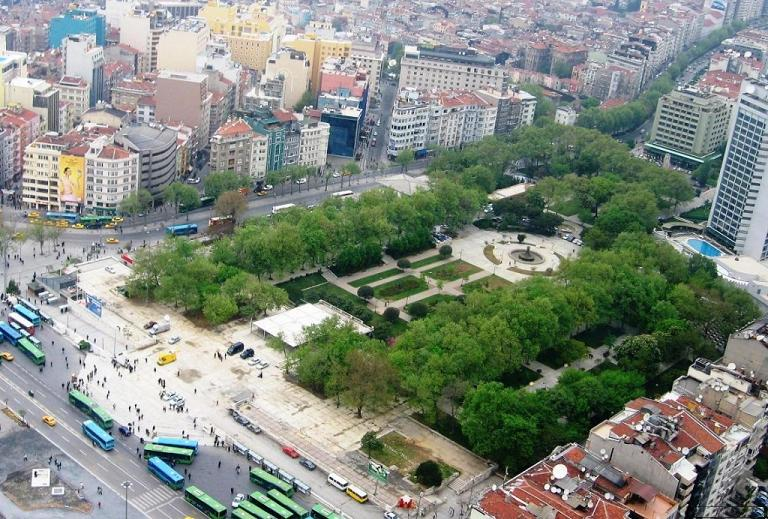
\includegraphics[scale=0.28]{Gezi_Parki.jpg}
  \caption{Gezi Parki before the protest. One of the few green spaces next to
  the Taxim Square and Istiklal Street.}\\
\end{marginfigure}

\begin{quote}
  We do not mean to suggest that social movements are everything and sufficient in themselves, but they do present a powerful ontological substance, and this nature of the movements must be understood before we can properly frame our contemporary political problem. The movements that interest us often have a Carsic nature; that is, they flow sometimes in full view and then descend for periods into subterranean channels, but together they nonethe­ less generate an accumulation of practices and subjectivity.

  -- \cite[67]{hardt2017}
\end{quote}

While the analysis of Erdoğan's rise to power through the AKP and the complex dynamics between secular and religious factions in Turkey often sparks debate, interpretations vary significantly. Some view the AKP's ascent as a simple representation of a different demographic within the country \parencite{defneover2017}, while others interpret it as a covert coup against the founding principles of the republic or as an overlay of religious conservatism atop Turkey’s entrenched nationalism. This paper, however, does not aim to dissect the nature of the regime. Instead, our focus will remain on the organizational structure, development, and eventual decline of the Gezi Park movement itself.

It is clear that, by the time of the Gezi protests, a series of politically provocative events had intensified public dissent against the AKP, which had been in power for over a decade. In the three years leading up to the protests, from 2010 to 2013, a multitude of protest movements emerged, each reflecting different grievances across various sectors of Turkish society. During this period, student movements and secular middle-class protests were triggered by police actions during Republic Day celebrations, and there were public outcries against the prosecution and detention of military officers in the controversial Ergenekon and Balyoz trials. Kurdish political prisoners engaged in hunger strikes demanding peace negotiations and an end to the isolation of Abdullah Öcalan, while demonstrations also broke out against the detention of academics, journalists, and politicians associated with the Kurdish movement.

Further protests erupted in response to tragic events like the Roboski massacre and the Reyhanli bombings, while nationalist groups staged rallies against peace talks with the Kurds. Commemorative marches for the assassinated journalist Hrant Dink, May Day protests, and anti-war demonstrations against involvement in Syria also took place. Additionally, there were movements advocating for secular education in opposition to new educational reforms and protests against urban renewal projects that threatened historical landmarks such as the Emek movie theater and Inci patisserie. Various professional groups protested poor working conditions, the detention of journalists, job insecurity, subcontractor regulations, and disputes over collective contracts. Activists also rallied against internet censorship, abortion bans, violence against transgender individuals, and the construction of nuclear and hydroelectric power plants. This vast array of protests highlights the multifaceted opposition to the AKP, driven by a diverse set of issues rather than a single unified agenda \parencite[see 211]{defneover2017}.

On May 28, 2013, a small group of protesters initiated a peaceful demonstration at Istanbul's Gezi Park, aiming to protect the green space from destruction as part of the municipality's urban development plans. Although the Gezi movement began as a defense of this small park near Taksim Square, it quickly transformed into a direct confrontation against the prevailing regime in Turkey. Over the next three days, what started as a local environmental protest rapidly escalated into a broad-based mass movement. Initially emerging as a grassroots initiative to protect a cherished green space in Istanbul, the Gezi movement was sparked by the Istanbul Metropolitan Municipality’s controversial “Taksim Pedestrianization Project” in 2011, which proposed demolishing Gezi Park to reconstruct a historic Ottoman barracks.

In response to this plan, three key civil society organizations—Taksim Platform (Taksim Platformu, TP), Taksim Solidarity (Taksim Dayanışması, TD), and The Association of Taksim Gezi Park (Taksim Gezi Parkı Derneği, TGPD)—were established to oppose the park’s destruction. These groups coordinated a range of awareness-raising and advocacy efforts, such as the “Ayağa Kalk” (Rise Up) campaign, organizing public events, circulating petitions, and issuing press releases. These actions laid the groundwork for the massive protests that erupted in May 2013, showcasing a collective response to the government’s increasingly authoritarian tendencies \parencite[213]{defneover2017}.

\begin{marginfigure}

  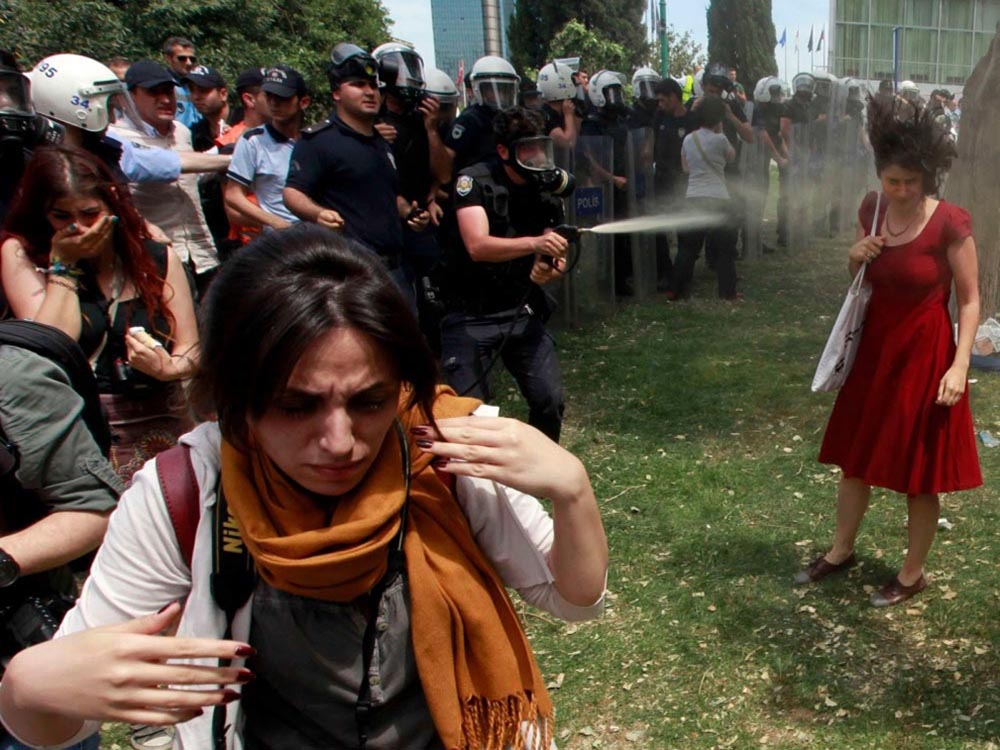
\includegraphics[scale=0.15]{Day1_1.jpg}
  \caption{Woman in Red: One of the most famous photos from the first day of the Protest. The protest form at the first day was reading books to the police.}\\
\end{marginfigure}

The Gezi movement was marked by its remarkably diverse coalition, encompassing a broad spectrum of societal groups, including environmentalists, secular nationalists, feminists, LGBTQ individuals, Kurds, Alevis, other minorities, anti-capitalist Muslims, radical left-wing groups, and even football supporters. A particularly notable example was the involvement of Çarşı, the core fan group of Beşiktaş, which played a prominent role in the clashes. Despite this wide array of participants, the Gezi movement quickly became associated with seemingly apolitical young men and women, predominantly students and white-collar workers \parencite[202]{agartan2018}. This demographic not only emerged as the most visible group on the ground but also began to shape the movement's direction, reflecting their unique characteristics and concerns.

Understanding this demographic shift requires considering Turkey’s history of protest, which was significantly stifled following the 1980 military coup that aimed to suppress the Marxist movement and the Kurdish left. In the aftermath, social movements in Turkey have been predominantly influenced by leftist organizations that survived this period of intense repression. For many young participants in the Gezi movement, confronting authority was an entirely new experience, lacking both the historical context and previous opportunities for political engagement \parencite[see 71-73]{tufekci2020}. These young people primarily came from families with a tradition of supporting the CHP (Republican People's Party), Turkey’s oldest political party founded by Mustafa Kemal Atatürk. While the CHP positions itself as a center-left party, it has often been criticized for its nationalist stance and has functioned as the main opposition party since the inception of the AKP regime. For many of these young protesters, loyalty to the CHP went beyond mere political alignment—it was deeply rooted in family heritage and historical involvement. Their families were likely politically active before the 1980 coup, often supporting government actions and the military against Kurdish minorities or communist organizations. Although these observations involve some assumptions, the crucial point is that the majority of those who joined the Gezi movement were experiencing direct confrontation with the government and police for the first time, marking a significant shift in political engagement for this demographic \sidenote{Diverse sources can be cited, albeit not academic.}.

The Gezi protest was particularly well-organized in terms of logistics. Beyond the well-maintained tent area—upheld primarily through self-responsibility and voluntary efforts to keep the space clean and orderly, a critical matter given the initial environmental motivations to save the trees and preserve one of the last patches of green space in an increasingly \textit{concretized} Taksim Square—there was a rapid establishment of a robust support system. Within just a few days, the movement had set up "three hot meals a day, clothes and blankets, an operating clinic with basic capabilities, a street library stocked with books, workshops on a variety of topics, and a steady stream of donations, volunteers" \parencite[51]{tufekci2020}. Additionally, a highly effective communication network, primarily utilizing Twitter, facilitated swift information dissemination and coordination.

This extensive logistical network significantly enhanced the agility of the protest community, enabling them to swiftly respond to sudden police attempts to evict the core group from the park. Moreover, there was a continuous effort to combat misinformation and corruption online, reflecting the movement’s multifaceted approach to resistance (see ibid.). As police brutality escalated, cooperation among protesters became more organized, particularly in managing the effects of excessive tear gas and providing medical assistance to the injured. Innovative, makeshift solutions, such as homemade mixtures to neutralize tear gas effects, modified gas masks, and tutorials on self-protection against police aggression, were shared widely, demonstrating a strong sense of solidarity and mutual aid among the participants.

\section{H1; Derepresentation and Failed Factions}
\begin{marginfigure}

  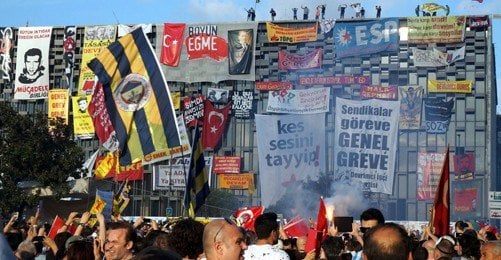
\includegraphics[scale=0.3]{bayrak.jpg}
  \caption{Flags on AKM (Ataturk Cultural Center) next to the Gezi Park during
  the resistance}\\
\end{marginfigure}


Revisiting the initial hypothesis, we must consider whether distinct factions were formed within the Gezi movement or if the movement fundamentally resisted such divisions. From the outset, Gezi did not lack representation in a dyadic sense. Even before any formal representative claims were made, both the regime and the opposition primarily perceived the Gezi Park community as an extension of the CHP's support base. However, the reality on the ground was far more intricate. The movement encompassed a multitude of leftist organizations, spanning from radical groups, including some with guerrilla histories \sidenote{For example, the PKK (Kurdistan Workers' Party) also had a presence at Gezi.}, to more moderate social democratic entities, and organizations focused on specific issues such as environmental activism.

This diversity was, in part, a reflection of the region’s complex history of ethnic marginalization and the persistent cultural and religious conflicts that often resulted in territorial and identity-based tensions. Additionally, the legacy of the leftist uprising and the subsequent military coup of 1980 played a significant role in shaping the landscape of activism in Turkey, leading to a proliferation of organizations and movements vying for influence and representation within the Gezi protests. A variety of NGOs and activist groups emerged, each attempting to assert leadership or claim the movement’s representative voice, demonstrating the multiplicity of interests and agendas that characterized Gezi \parencite[see 229]{defneover2017}.

As the protest gained momentum, there was a marked increase in the visibility of various political parties and their symbols at Taksim Square and Gezi Park. Within a short period, the protest space was filled with flags and banners representing a range of parties and leftist factions \parencite{2023v}. This sudden influx of partisan symbols was met with strong resistance from the Gezi community for several reasons. Primarily, Gezi protesters were continuously subjected to profiling and stigmatization by both the ruling regime and other political groups. The AKP, under President Erdoğan, along with conservative factions, accused the protesters of engaging in immoral behavior, aligning with terrorist activities, acting as the aggressive arm of the opposition, or being manipulated by figures like George Soros. Concurrently, opposition parties sought to co-opt the movement by framing the protesters as their supporters, despite the widespread dissatisfaction within the Gezi community regarding the lack of substantial support from these parties \parencite[see 100-110]{tufekci2020}.

In response to these dynamics, Gezi protesters actively endeavored to disassociate themselves from any form of imposed representation or political affiliation. This effort to maintain an untainted identity became particularly pronounced when partisan flags began to appear throughout the protest area, triggering a vehement backlash from many participants. The unrepresentative claims of the Gezi movement were specifically aimed at factions that were perceived to be attempting to impose their presence on the movement. Protesters called on these self-appointed representatives to "lay down their arms," signaling a broader rejection of traditional political affiliations and the concept of representation. This was not merely a rejection of alignment with the small leftist parties; it was an assertive disavowal of any external attempts to co-opt the resistance. Public statements were issued condemning what many saw as provocative efforts to hijack the movement. Consequently, protesters demanded that these groups either withdraw from the area or remove their flags, a request that most of the leftist factions ultimately respected.

This experience, however, generated a deeper anxiety within the Gezi movement about becoming associated with any particular faction or undergoing a process of factionalization. I argue that this aversion to factional identification was one of the key factors that hindered Gezi protesters from articulating demands that went beyond the immediate objective of stopping the construction plans. By avoiding factionalization, the movement may have preserved its image of unity, but it also limited its capacity to formulate a broader, more transformative political agenda.

\section{H2; Adopted referent "çapulcu"}

The representative issue that both Hayat \parencite*[1041]{hayat2022} and Tüfekci \parencite*[72]{tufekci2020} identify as contributing to the end of the Gezi movement was the failure to establish a coherent form of representation, which allowed the regime to select representatives on its own terms. While this is certainly a significant factor, the deeper reasons for this failure extend beyond the immediate concerns of the movement itself and are rarely examined. I argue that the fundamental issue underlying this failure was the lack of triadic representation—the Gezi community was unable to create a cohesive image of itself without defining itself merely by opposition to everything it rejected. In essence, Gezi was a failure in constructivist terms; it failed to construct a unified identity or coherent strategy.

\begin{figure*} 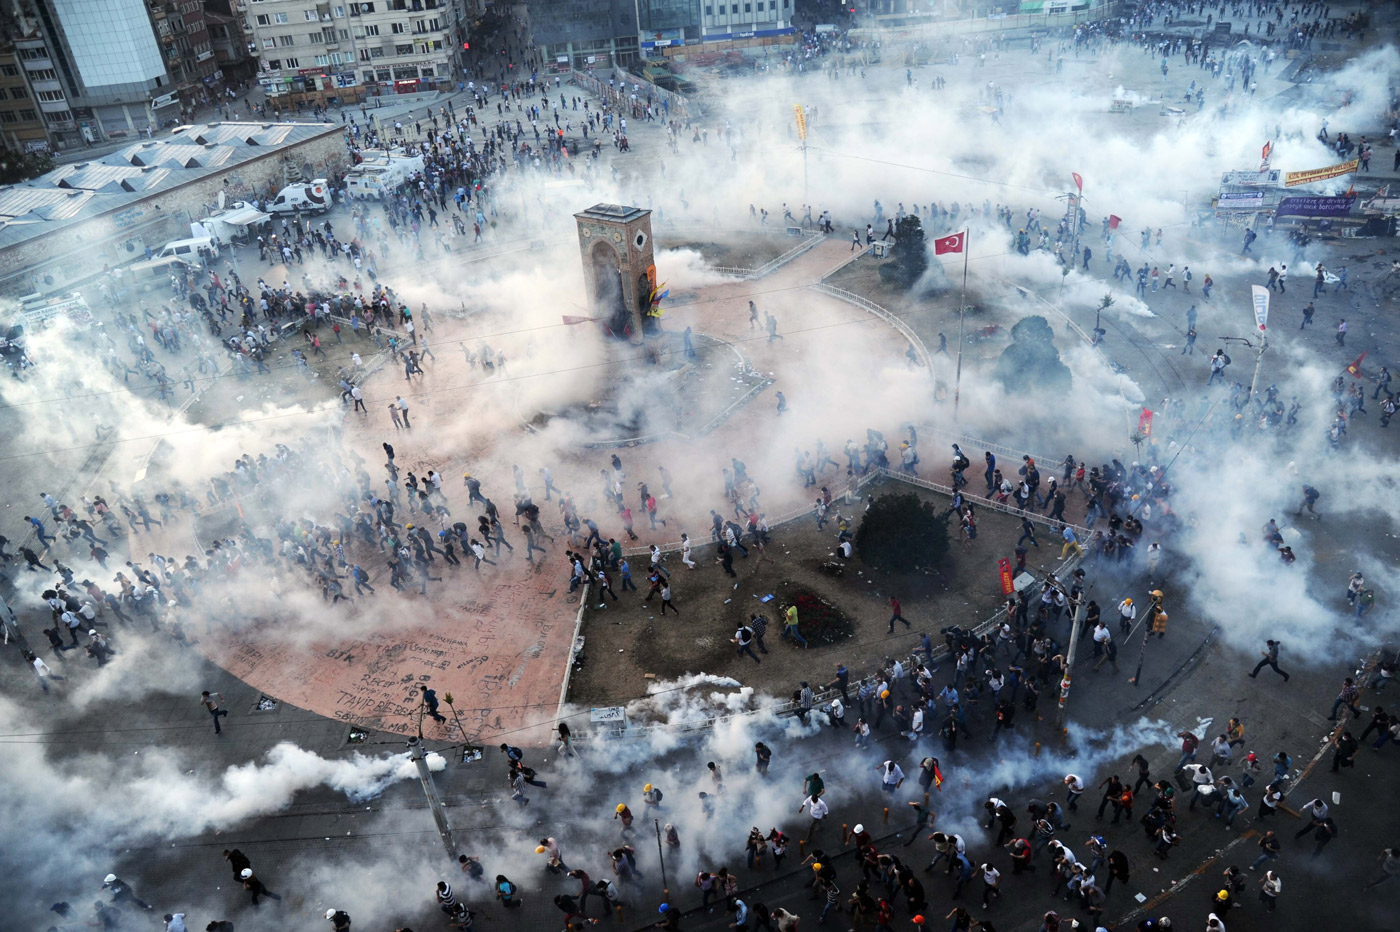
\includegraphics[scale=0.32]{teargas.jpg} \caption{Extensive tear gas use at Taksim Square during the Gezi Protests}\ \end{figure*}

As discussed in the previous chapter, my argument centered on the idea that forming a referent is a critical step in the development of a political constituency, whether through the construction of a representative or by exploring the community’s self-identity. In the case of the Yellow Vests, I argued that their reliance on unrepresentative claims and the broad, self-defined image of the "citizen" was too vague to foster any meaningful factional development within the movement. The situation at Gezi was even more intricate. Unlike the Yellow Vests, the Gezi protesters could not unite around a historical characterization, such as the Sans-Culottes, because they were unable to align themselves with any of the existing leftist parties or their historical legacies. All historical references available were perceived as too radical or incompatible with the movement’s ethos.

An illustrative example of this is the figure of Deniz Gezmiş, a revolutionary who was executed by the military junta following the 1980 coup due to his militant political activities. His presence and ideology were palpable at Gezi Park, and his blend of patriotism and socialism made his ideas more palatable to some participants than those of other historical revolutionaries. Yet, despite his relative appeal, Deniz Gezmiş was still seen as a guerrilla who had taken up arms against the state—a stance that many within the Gezi movement, even as they clashed with police, were reluctant to fully embrace. The secular Kemalist majority at Gezi found it difficult to fully associate with any explicitly anti-state or anti-police ideology.

However, a defining concept was unexpectedly provided to them by the regime itself, specifically by Erdoğan. In one of his balcony speeches, Erdoğan referred to the protesters as "çapulcu," a derogatory term roughly translating to "looters" or "worthless/lumpen punks." This pejorative label was swiftly co-opted by the protesters, who turned it into a badge of honor and a unifying identity. The term "çapulcu" became a referent that could encompass all those resisting Erdoğan’s regime \parencite[2]{ulug2019}. It quickly gained popularity among nearly everyone opposing the regime and remained synonymous with the opposition support base for years. In many ways, it was the only characterization that emerged as a lasting legacy from the Gezi Movement. Unlike other historical movements that had clear identities such as the Sans-Culottes, the Jacobins, or the Diggers, Gezi did not produce a comparable referent or a set of radical demands, nor did it have a means to enforce them, as both Hayat and Tüfekci have noted.

\begin{quote} What began as a local issue had become symbolically important nationally, and the government’s offer appeared to concede this. In the park, people voiced mistrust of the government, and many were unsure how to react. Some thought that this would be a good opportunity to declare victory. Some booed; others clapped. Some cheered; others jeered. The crowd was split. Unlike previous times when government plans had clearly been seen as illegitimate by majorities within the park, this proposition produced a division in the movement.

-- \cite[73]{tufekci2020} \end{quote}

Ultimately, the Gezi movement experienced what could be described as a tactical freeze. Despite the efforts to create an Agora-like space in the park to facilitate mass discussions, the movement’s momentum was waning. The lack of a coherent representational structure meant that the Gezi movement’s engagement with the government was largely dictated by the authorities. Representatives were chosen by government officials, starting with celebrities and then moving to an arbitrary group from the movement, but no radical demands were articulated or pursued by the end of the resistance.

\section{H3; Solidarity and \textit{Unity} at Taxim Square}

The Gezi Resistance ultimately managed to establish a robust network of logistics, planning, communication, and solidarity among various segments of society, which contributed to the relatively extended duration of the protest \parencite[51]{tufekci2020}. As highlighted in the previous section, a forum resembling an ancient Agora was also set up to deliberate on the movement’s demands from the government. Within the park, protesters initiated what they termed "small forums," encouraging individuals to break into smaller groups to discuss the government's proposal. This represented the first structured attempt to facilitate open dialogue among all participants during the protest. However, the process was somewhat chaotic, with no clear guidelines on who could participate or how decisions would be made. Despite the lack of formal structure, there was significant enthusiasm for these discussions, as many saw this as a potential turning point for the movement.

Participants formed several smaller groups, clustering around various spots like trees, tents, and open spaces, since a single large gathering was impractical. Even these smaller assemblies, however, were quite substantial, often comprising hundreds of people. The discussions continued for nearly nine hours, underscoring the deep engagement and commitment of the protesters. Yet, as these dialogues were unfolding, the tension was further exacerbated by the governing party’s decision to hold a rally in another part of Istanbul, demonstrating their intent to counter the protest with a show of strength. The following day, confusion and disorganization persisted. Although the forums had lasted a long time, the absence of established decision-making mechanisms meant that no clear conclusions or strategies emerged from the discussions \parencite[73]{tufekci2020}.

I contend that even in highly successful rhizomatic organizations, there is a crucial need to streamline specific interests into distinct factions to foster productive discourse. While the formations within social movements may not closely resemble the structure of a political party, they function as proto-party formations, laying the groundwork for more formal political engagement. Movements that fail to encourage the formation of factions face two significant risks:

\begin{enumerate} \item Ambiguity in Goals: By creating a broad identity that vaguely appeals to the entire movement, there is a risk of diluting specific objectives, leading to a lack of clarity and focus in the movement’s goals. This ambiguity can hinder the ability to articulate a coherent strategy or negotiate effectively with authorities or other stakeholders.

\item Silencing Minority Voices: Without the formation of factions, minority voices within the movement may be marginalized or overlooked. Factional representation can ensure that diverse perspectives are included in the decision-making process, potentially influencing the direction of the majority and enriching the movement's overall strategy and impact.

\item Tactical Freeze: A low confrontational discourse can eventually result in a tactical freeze, where the movement struggles to make decisive actions or adopt effective strategies. Without robust debate and conflict, the movement may lack the dynamism needed to respond to changing circumstances or to challenge the status quo forcefully. \end{enumerate}

Despite the collapsing movement without being able to scale up their goals, Gezi
has at least established saving the park. Gezi had been also an event as in Badiou's terminology, it has been a
rupture that led to the proliferation of
possibilities of new political subjectivities. The most prominent effect was to
mobilising (and also scattering along the way) a youth which was defining
themselves Kemalist which usually referred to a secuar nationalist, into a
non-apolitical direction. For many, just the clashes with the police gave enough
food for thought for deliberate political activity. But there are more
concerete results than this; after saving a \textit{public thing} in Honig's
terminology, Gezi protesters went building a new public space by first
transforming a squat building in a small neighborhood called Yeldeğirmeni into a
culturall centre, they continued transforming the whole neighborhood
\parencite[see for example]{durgun2021}. And also experimented with new protest
forms like Duran Adam (Standing Man) whereas a man started protesting just by
standing days after Gezi protest that collected lots of support both on the
field and on social media \parencite[see for example]{verstraete2013}. The
examples can be extended, while in the social movements prevention of
factionalisation for the sake of more inclusivity leads to a potential
paralysis, rhizomatic organisations opens a production of new subjectivities and
organisation forms.


\chapter{Conclusion and Outlook}

The Gezi Resistance provides a compelling case study for examining the complexities of political representation and organizational structures within contemporary social movements. Through the theoretical lenses of Michael Saward's "Representative Claims," Samuel Hayat's "Unrepresentative Claims," and Michael Hardt and Antonio Negri's theory of Assembly, this paper has explored how the movement's dynamics were shaped by various approaches to representation, inclusivity, and leadership after introducing and analysing the cases and arguments those authors Have been publishing.

The Gezi movement’s inability to establish a coherent form of representation (highlighted by its avoidance of factionalization and failure to produce a unifying referent) underscores the challenges faced by leaderless and decentralized movements. While these movements often emphasize inclusivity and direct participation, neglegtion of the faction forming and representation of different interests and goals leads to an ambiguity both regarding the identity and goals of the movement. I claimed it to be the real reason the \textit{tactical freeze} happened at the end of the movement.

I have also argued the main cause of this is inability of production of referent(s) in the movement which is especially important in the movements denying Weberian type of representation. As a self-constructivist process and in the \textit{Darstellung} form of representation, defining different images belonging to different factions standing for different goals might prevent a broader definition of a single referent for the whole movement which is while inclusive, can be also pacifysing for the movement by its tendency to tamer goals. 

Furthermore, although factionalisation is important, I have argued that in the
case of Gezi, the lack of factionalisation not necessarily lead to the
prevention of the creation of new subjectivites, and organisational forms after
the movement which was one of the arguments of Hardt and Negri, in case an
effective horizontal organisation and solidarity network is established.
    \printbibliography
\end{document}
